\section{Qualitative Evaluation}

The interaction paradigm of SimpleSpeech was tested in a qualitative assessment to determine (1) the practicability of a lightweight text-based audio editor, (2) the effects of minor transcription errors on audio consumption and production, and (3) the implications of being able to edit audio in an asynchronous online discussion.

Participants were introduced to the functionality of the system, then given two untimed tasks. 
First, to simulate an asynchronous audio discussion, the test users were asked to read an audio comment left by the previous tester and create an audio response. 
Next, they received a different, textual prompt and created an audio comment which would be consumed by the next user. 
In both cases the user was asked to edit their recordings to be polished and clear.
The participants were interviewed at the end of the test over three general topics: (1) comparing the hybrid editor with conventional text editing, (2) comparing the discussion component with a text-based or face-to-face conversation, and (3) any user experience issues that occurred during the study. 
Afterwards, the interviews were transcribed, conversational elements filtered out, and the remaining sentences analyzed via two-step coding (open coding followed by flat coding). 

The sample for the study consisted of 9 test subjects (4 male, 5 female; henceforth denoted $P_1, P_2, \ldots, P_9$). 
All participants were native English speakers. 
Two individuals, $P_2$ and $P_3$, were professional media editors who provided technical feedback and a comparison to pure audio editing; the remainder were interns and high school students.

\subsection{Results}
The coding process for transcripts resulted in the following themes identified from the user feedback:

\emph{The text-based proxy provides sufficient control over elementary editing to supersede waveform manipulation.}
Most non-professional users felt SimpleSpeech gave them ``plenty of control'' over the editing process ($P_4,\,P_5,\,P_6,\,P_8$). 
The professional editors did note that most people in their field would not find this software adequate for their needs; but, as $P_2$ conceded, the intended market users ``don't have to play with the settings which is why they don't use a professional audio editor.''
Most participants characterized the editing experience as being a text-focused one, suggesting that the translation to text was in fact a useful proxy for editing audio. 
The text modality was described as ``more accessible, more doable'' than pure waveform editing, which could be ``scary for people who don't do video stuff'' ($P_3,\,P_7$). 

\emph{The primary use of lightweight voice editing is to make fine-grained rather than large-scale adjustments.}
The most commonly-used manipulation during the qualitative study was the removal of disfluencies ($P_1,\,P_2,\,P_4,\,P_5,\,P_7$), followed by space deletion ($P_2,\,P_3,\,P_5,\,P_6,\,P_8$). 
Only $P_1$ and $P_8$ edited large chunks of audio by deleting or rerecording, and $P_8$ reported doing so only to improve the smoothness of a smaller change in a sentence.
Perhaps because SimpleSpeech was presented as a tool to be briefly used to ``clean up'' recordings, participants focused on removing the ``embarrassing'' and ``awkward'' sounds ($P_1,\,P_5$).

\emph{Transcription is a helpful aid for listening to audio comments despite occasional errors.}
In many cases, the transcription proved to be an essential element of both the production and the consumption interfaces. 
To determine the effect of errors in the textual representation, the previous participants' comments were displayed to users with an unedited ASR transcript instead of the polished, human-edited one. 
Despite the occasional errors, users still found the ASR transcription to be helpful in allowing them to ``see all the points they were making instead of having to remember them'' ($P_4,\,P_6$). 
For some users, the transcription caused no problems in comprehension, while others experienced errors that required them to pay more attention to the audio ($P_8$). 
On the whole, ASR succeeded in ``getting the basic idea across'' ($P_3$) but could not stand alone without the original recording. 
In the editing scenario, most users agreed that the transcription functionality was ``overall quite accurate'' if they spoke clearly enough ($P_1,\,P_3,\,P_4,\,P_5,\,P_6,\,P_7,\,P_9$). 

\emph{The linearity of audio leads to a pressure to organize one's thoughts during recording.}
In some participants we also observed pressure associated with the audio production process. $P_4,\,P_7,$ and $P_9$ described a ``psychological sort of ... need to get it all out, and the fact that it won't necessarily be as organized there.'' 
Another tester, $P_5$, had ``a tendency to get like a blank slate'' in which he ``couldn't think of anything to say.'' 
The elevated mental task load that $P_5$ describes could be inherent in oral discussion; $P_9$ noted that ``[it] might just be the fact that I was recording,'' and in fact ``editing would make it nicer.'' 
Because this phenomenon was present despite the ability to edit and because it has not been explored in the literature to our knowledge, we decided to analyze the task load aspect of using SimpleSpeech in the quantitative study.

\emph{Awareness of the recipient and the editability of the audio drive up the quality of contributions.}
Interestingly, the participants' awareness of their audience and the ability to edit tended to drive up the quality of recordings.
Four users mentioned the formality of recordings using the software of their own volition or prompted by a question about pressure ($P_1,\,P_5,\,P_7,\,P_9$). 
$P_8$ described the situation as ``an expectation'' to edit, given that ``I know that I've had that opportunity and someone else would know that I had that opportunity.'' 
The speakers' inclination to consider their listeners is exemplified by $P_9$, when asked why she was motivated to edit her messages:
\begin{quote}
	Personally I'm editing to express myself a little more in a polished way when I'm writing.... especially if I know someone else is going to review it and be able to respond, I want to make sure I'm as clear as possible and as concise in a way that doesn’t really come across when I'm talking.
\end{quote}
Listening to another participant before initiating their own comment was likely a factor in determining the users' performance, since the exposure ``gave ... an understanding of how long of a comment, or what kind of direction people were trying to take the discussion'' ($P_9$). 
Editing contributed to the increased quality as well: ``Since you have the ability to edit things, it feels like you're talking to somebody who's prepared a point or a conversational view'' ($P_5$). 
We chose to explore this phenomenon quantitatively to determine if it was real or simply perceived by the speakers, and to what extent it was affected by the ability to edit.

\section{Quantitative Evaluation}
For our second, quantitative experiment, we intended not just to assess the efficacy of SimpleSpeech in particular, but also to measure the usefulness of audio editing tools in general for educational discussions.
Participants in the study were given two task parts in random order: recording messages without editing functionality (the No Editing, or NE task) and using SimpleSpeech (the Editing, or E task). 
Both tasks were presented in a similar UI, except that in the NE part the transcript area was disabled to prevent editing.
Each task involved participation in two ``discussion threads'' on an online forum; each of these subtasks entailed reading one of six possible prompt statements, listening to another person's opinion on the issue, then producing an original response.
(Before starting the E part, participants were given a standardized tutorial to learn how to edit using SimpleSpeech.)

The initial ``stimulus'' recordings for each of the prompt statements were generated by a group of five initial volunteers. 
Since the qualitative study had indicated the possibility that prior exposure to other individuals' messages could affect users' perception of formality in the discussion, we divided the stimuli into formal and informal sets. 
Half the participants of the study (Group A) received only formal recordings, while the other half (Group B) received only informal ones.
We hypothesized that since in the qualitative study the participants created more formal messages because of exposure to similar comments, the participants in Group A would 

The criterion used for formality was the F-score, a measure of contextuality introduced by Heylighen and Dewaele in 2002 \cite{heylighen}.
The F-score is a purely textual metric based on the frequencies of various parts of speech in a text: nouns, adjectives and prepositions decrease the contextuality and increase the F-score since they are independent of the circumstances around the text, while deictic words such as verbs, adverbs, pronouns, and interjections increase contextuality and decrease the F-score. 
For our stimulus recordings, the initial participants were asked to plan and edit some of the comments and improvise on the others.
After splitting the resulting messages by formality, the average F-score was 53.7 for the Group A messages and 49.4 for the Group B messages, reflecting the greater contextuality of the recordings produced on-the-fly.
Group A stimuli also tended to have longer words than those for Group B (4.62 versus 4.38 letters) and tended to be more concise (113 versus 193 words).
After obtaining and categorizing these messages, the voices were anonymized by adjusting the pitch randomly.

After each task, the NASA Task Load Index (NASA-TLX) questionnaire was used to quantify the pressure or mental task load of producing a voice message \cite{nasatlx}. 
NASA-TLX is a subjective analytical tool measuring task load along six dimensions: Mental Demand, Physical Demand, Temporal Demand, Performance, Effort, and Frustration Level. 
After rating the level of each aspect of mental workload from 1 (least workload) to 20 (greatest workload), the subject is asked to compare the scales pairwise to produce a weighted TLX value representing the overall pressure during a situation. 
Participants in the study completed the TLX procedure once after each task to obtain comparisons between the mental workload induced by no-editing and editing situations.

The quantitative study was conducted at a small public high school, with x students and x teachers.

\subsection{Results}
The data collected in the quantitative study fell into three categories, which we will discuss here individually.

\subsubsection{Utilization of Editing Features}
As in the qualitative study, most participants appreciated and took advantage of the ability to edit their messages.
On average, users made about 17 edits to each voice message, consisting of inserting a new recording, inserting a pause, deleting words, or deleting a pause. 
Of these changes, the vast majority were subtractive: 7 word deletions and 6.3 pause deletions per message.
This was again consistent with the findings of the earlier study, which had shown an inclination to remove disfluencies and ``awkward'' hesitations from the recordings.

Ideally, participants in the E task would have edited both the transcription and the voice to be free of errors, but due to time constraints on participation time we discouraged the users from correcting transcript errors (which turned out to be more numerous than expected, especially because of the conversational style).
Incorrect transcriptions were problematic for editing in general: Since the associated timestamps were also incorrect (see Software Design), the edits on that segment of audio could produce undesirable results. 
Transcript errors fell into the following general categories:

\begin{itemize}
	\item \emph{Incorrect word for the same time interval.} 
	This was the most common type of error, especially for disfluencies (``um'' transcribed as ``I'm''). 
	It was also the easiest type of mistake to correct.
	\item \emph{Multiple words in the same time interval.}
	These errors would also be fairly easy to correct using SimpleSpeech, by summing together the appropriate word timestamps.
	\item \emph{Multiple words captured over a larger time interval.}
	These errors were fairly uncommon, but when they did occur they were detrimental to editing.
	\item \emph{No word captured for the time interval.}
	In this type of mistake, the timestamp for a word was simply registered by the ASR service as a pause.
	To avoid participants accidentally deleting these timestamps thinking they were pauses, we stressed to them during the tutorial to play back the recording before editing it. 
	Despite this, users did occasionally delete green pause tokens that contained speech, perhaps reflecting a perceived disconnect between the transcription and the audio source.
\end{itemize}

A few participants found the mechanism to edit the transcript (pressing Return) somewhat counterintuitive. 
When it was presented in the tutorial, at first these participants tried to use the Delete key on the token they wanted to edit, resulting in the permanent deletion of the word and its corresponding audio. 
The emphasis in the tutorial that the Delete key deleted the audio permanently did help other participants avoid making this mistake.

Another misconception we observed in a few participants was a tendency to treat SimpleSpeech as a dictation tool. 
The two primary behaviors associated with these users were pausing for long periods of time during recording sessions and not playing back the messages during editing. 
Furthermore, their inclination after stopping a recording session was to go back and correct transcription errors so that the visual representation made sense.

\subsubsection{Task Load}
Since the NASA-TLX scale is subjective, it does introduce variability between participants due to the differences between their perceived skill at the task \cite{nasatlx}. 
For instance, one participant could rate the recording task at a 3 out of 20, while another could rate the very same task at a 15.
Therefore, the strongest comparisons of task load were made in the within-subject dimension, which was the ability or inability to edit.

Overall, the students reported significantly \emph{lower} levels of mental task load or pressure during the E task than the NE task (mean 8.7 compared to 10.8, $p<0.02$). 
The values for the individual components of the TLX, shown in Table \ref{tab:table1}, yielded the following contributory dimensions on the TLX questionnaire:

\begin{table}
	\centering
	\begin{tabular}{r c c c}
		\multicolumn{3}{c}{\textbf{Students} ($N=16$)} & \\
		\toprule
		Task			& \textit{E} & \textit{NE} & \\
		Mental Demand   & 9.6      & 11.1 		   & \\
		Physical Demand & 3.7      & 2.6           & \\
		Temporal Demand & 7.8      & 10.5          & * \\
		Performance     & 8.3      & 10.0          & * \\
		Effort          & 9.1      & 11.6          & * \\
		Frustration     & 7.8      & 8.9           & \\
		\midrule
		Total (weighted)& 8.7 & 10.8 & * \\
		%& \multicolumn{2}{c}{$p=0.011$} \\
		\bottomrule \\
	\end{tabular}
	\caption{The mental work load ratings reported by students, along with the total task load index values. (* -- $p<0.05$)}~\label{tab:table1}
\end{table}

\begin{itemize}
	\item \emph{Temporal demand}. Students rated the temporal demand at 7.8 for the E task, compared to the NE rating of 10.2. 
	As described by the TLX form, temporal demand refers to ``time pressure ... due to the rate or pace at which the tasks or task elements occurred'' \cite{nasatlx}.
	Students verbally described the increase in time demand reported on the TLX in terms of having to think of words to say quickly, with the knowledge that every second not filled with speech would be an embarrassing silence.
	\item \emph{Performance}. Students felt significantly more concern about the quality of their messages in the NE task, rating it at 10.3 compared to 8.0 for the E task. 
	Just as the participants in the prior qualitative study had articulated a desire to make their messages better for the sake of their listeners, the students also evidently wanted to improve their recordings in the NE task. 
	The inability to do so resulted in the elevated task load due to performance, while for the E task the stress along that dimension was lower because they were afforded the chance to correct their mistakes.
	However, it is worth noting that even despite the capability to edit, the student participants still rated Performance close to the middle of the scale, perhaps representing self-consciousness or comparisons with the stimulus recordings.
	\item \emph{Effort}. Similarly to performance, students reported having to work harder in the NE task to accomplish the task to their desired level (rated 12.1 compared to 9.0 in the E task). 
	This increased effort could correspond to the additional mental activity which had to be expended in order to generate speech fluently and without excessive hesitation.
\end{itemize}

The teachers also reported slightly lower workload levels, as shown in Table \ref{tab:table2}, but this difference was not significant.
In fact, 7 of the 13 participating teachers actually rated the E task as requiring a higher workload than the NE task.
This subset of the teachers, 5 of whom were in Group A, reported an average task load greater in the E task than the NE task for \emph{all} dimensions, especially Mental Demand, Performance, and Frustration.
The reason for this rating, these teachers explained, was that the availability of the editing tools caused them to feel more worried about their performance and expend more effort to edit without sacrificing the existing fluidity of their messages.

Interestingly, this particular group of teachers produced more formal messages than the other teachers (mean F-score 56.6 compared to 53.1 for the other teachers), with longer words (4.58 compared to 4.36 letters), and fewer disfluencies (13 per thousand compared to 21 per thousand).
Upon further inspection, the student participant group also contained members who similarly rated the E task as more demanding than the NE task, though fewer in number (4 out of 16); these students also produced much more formal messages than their peers (57.9 compared to 53.5). 
These participants could have had more experience speaking extemporaneously or felt less inclined to speak conversationally, ultimately leading to SimpleSpeech not being as useful to them.

Overall, the fact that the differences in workload varied so profoundly among teachers indicates that they were not as heavily affected by the ability to edit as the students, who clearly appreciated.

\begin{table}
	\centering
	\begin{tabular}{r c c}
		\multicolumn{3}{c}{\textbf{Teachers} ($N=13$)} \\
		\toprule
		Task			& \textit{E} & \textit{NE} \\
		Mental Demand    & 11.5 & 11.2 \\
		Physical Demand  & 4.0  & 3.2  \\
		Temporal Demand  & 7.8  & 9.9  \\
		Performance      & 8.2  & 9.5  \\
		Effort           & 10.0 & 10.4 \\
		Frustration      & 8.4  & 9.7  \\
		\midrule
		Total (weighted) & 9.5  & 10.6 \\
		& \multicolumn{2}{c}{$p>0.05$} \\
		\bottomrule \\
	\end{tabular}
	\caption{The mental work load ratings reported by teachers, along with the total task load index values.}~\label{tab:table2}
\end{table}

\subsubsection{Formality}
Contrary to the hypothesis that prior exposure to messages created using SimpleSpeech would affect the formality or linguistic traits of new messages, the F-scores of the participants' output varied independently of what group they were in.
As in the workload measurements, the average F-score for students was higher for Group A (55.83) than Group B (53.42), which is a considerable difference in terms of the F-score's scale but not statistically significant. 
The F-scores for teachers were almost distinguishable, with a difference of only 0.38.
In other words, the formality of the recordings was not affected by the stimulus message or even whether the participant was a teacher or a student.
Considering that the F-score measures contextuality between the speaker and the audience, and that its value was not affected significantly by the context given before the tasks, the principal source of variation in F-score was due to personal preference in the medium and scenario presented (recording a message to submit to an online forum discussion).

\begin{table*}
	\centering
	\begin{tabular}{r c c c c}
		\toprule
        & \multicolumn{2}{c}{\textbf{Students}} & \multicolumn{2}{c}{\textbf{Teachers}} \\
        \cmidrule(lr){2-3} \cmidrule(lr){4-5}
        Group                         & \textit{A}    & \textit{B}   & \textit{A}    & \textit{B}   \\
        Formality (F-score)           & 55.83         & 53.42        & 54.74         & 55.12        \\
        Word Length                   & 4.40          & 4.44         & 4.50          & 4.46         \\
        Disfluencies (per 1000 words) & 15.92         & 23.80        & 12.67         & 19.46        \\
        Word count                    & 100.66        & 140.47       & 155.38        & 127.00       \\
        Speaking rate                 & 130.39        & 114.75       & 136.58        & 139.01       \\
		\bottomrule \\
	\end{tabular}
	\caption{Various metrics representing the formality of the audio messages produced by each participant group.}~\label{tab:table2}
\end{table*}

\section{Formality Comparison}
Determining the formality of voice-based asynchronous discussions is a revealing indicator of this technology's potential applications, and one that has not been studied extensively.
The closest related studies have pertained to other forms of computer mediated communication (CMC), especially textual ones such as SMS, email, or Facebook posts.
For example, Kiesler, Siegel, and McGuire \cite{kiesler} found more equalized group participation and more uninhibited expression of opinions in synchronous text-based CMC than in face-to-face discussions.
Asynchronous CMC, similar to a discussion board, has also been shown to induce more prosocial behavior and, in fact, more informal communication styles over time than face-to-face \cite{walther}.
The same informality has been shown to be true for text messages and Facebook-style posts \cite{bilal}.
On the other hand, formality or politeness in emails generally increases as the social distance, status gap, and importance of a request increase \cite{cho}.

How asynchronous audio discussion fits into the complex hierarchy of social dynamics on various platforms is still unknown, so we conducted a comparative analysis of the voice messages composed during this study with several corpora of different media.
For comparison with written documents, we used several sections of the well-known Brown corpus to compile general categories of text: nonfiction, fiction, and technical (consisting of government documents, scientific articles, and news) \cite{brown}.
We obtained chatroom text from the \texttt{nps\_chat} corpus, face-to-face conversation data from the \texttt{webtext} corpus, and telephone data from the \texttt{switchboard} corpus, all available as part of the Natural Language Toolkit (NLTK) \cite{nltk}.
Finally, we also analyzed email communication in non-spam messages from the Enron corpus \cite{enronsent}, as well as Twitter posts \cite{twitter}.

\subsection{Results}
The results of this comparison, shown in Figure \ref{fig:formality}, illustrate the middle-ground that AAC takes relative to oral and written media. 
The least formal and most contextual corpora were those based on oral communication (with the notable exception of web chat messages), while the most formal and least context-dependent were the written texts, including email and Twitter posts. 
We will note three possible explanations for the formality of each medium based on the ordering of the corpora:

\begin{figure}
	\centering
	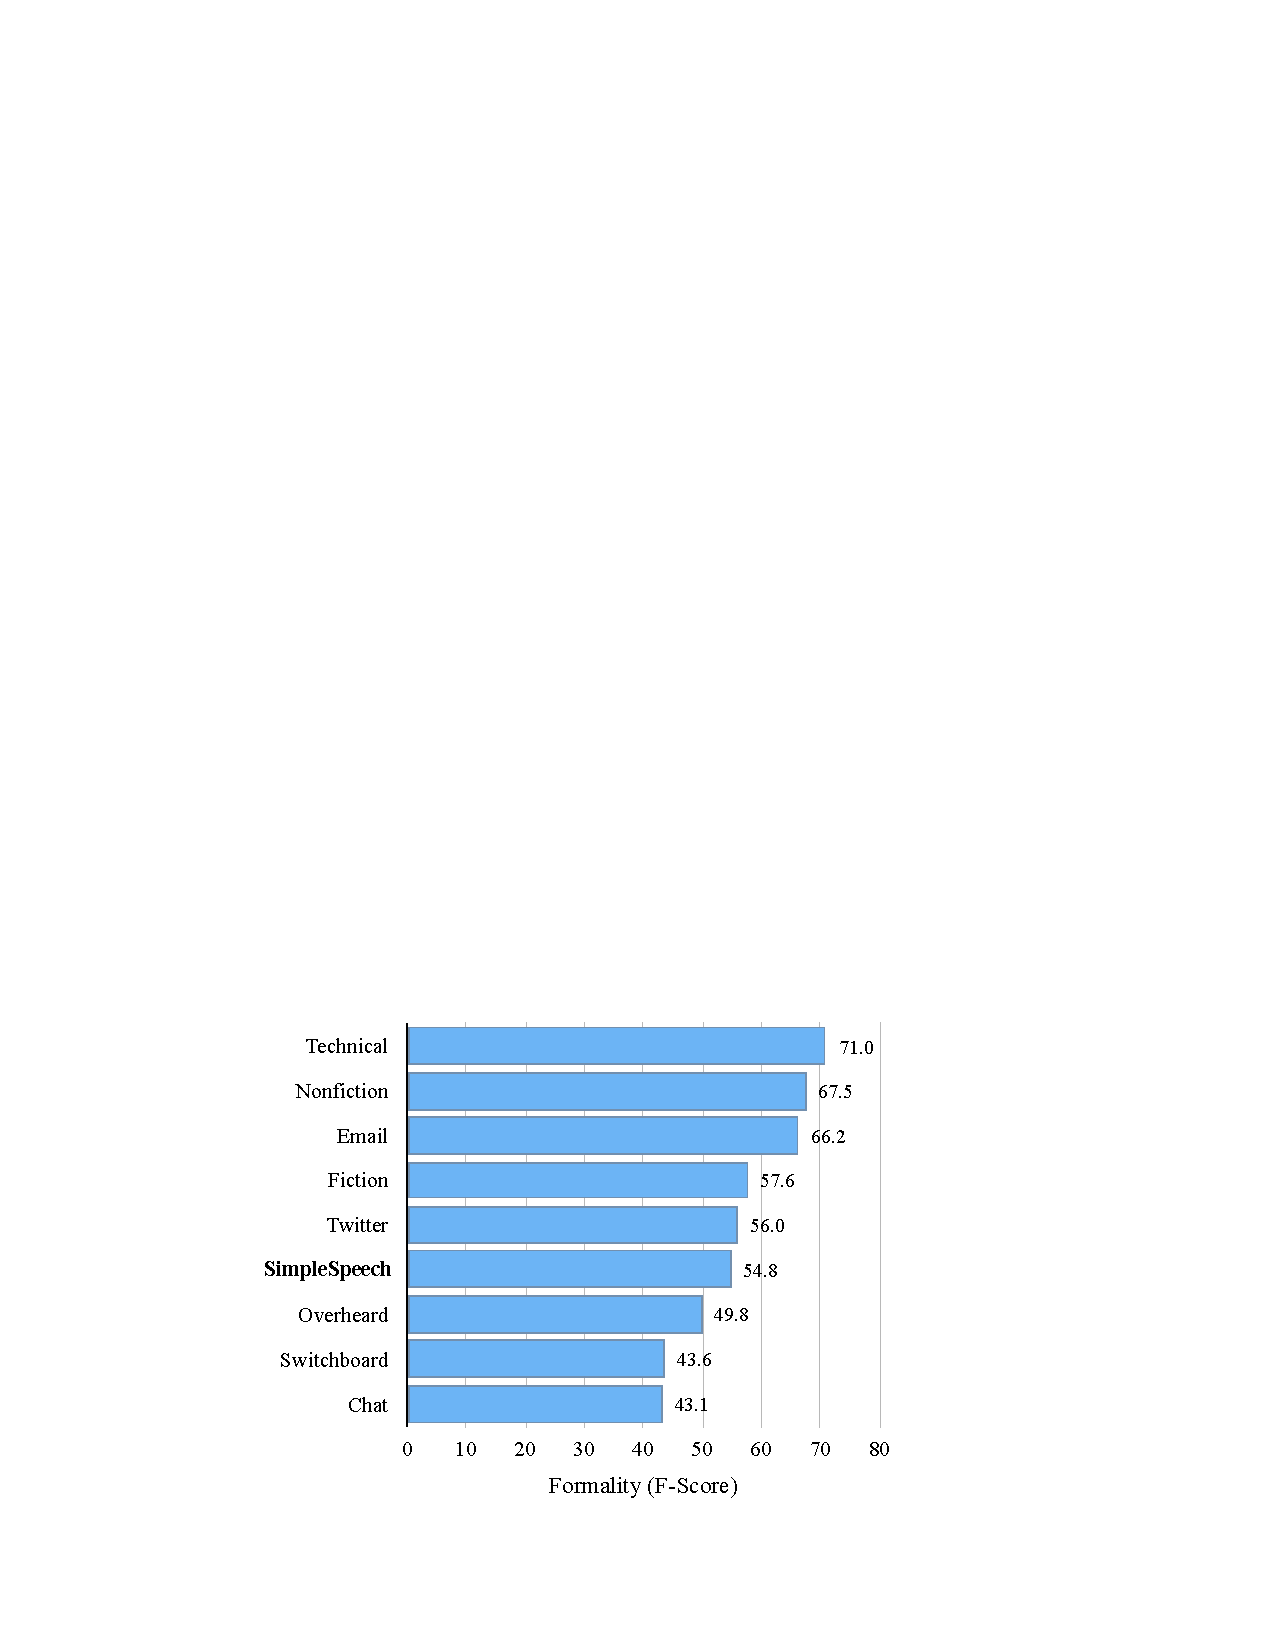
\includegraphics[width=\columnwidth,keepaspectratio]{figures/formality_comparison}
	\caption{The formality of corpora in different genre and media. The messages produced using SimpleSpeech during the quantitative study are intended to reflect general AAC discussion characteristics.}~\label{fig:formality}
\end{figure}

\emph{Speaker-audience relationship}. 
Since the F-score ultimately measures contextuality, it is reasonable that the chat and telephone corpora were the most contextual because the participants knew each other and were conversing on a one-to-one basis. 
On the other hand, the written forms of communication (with the exception of email) were less contextual because the audience was defined more loosely and not necessarily acquainted with the speaker.
The form of AAC studied here was more closely related to the latter condition (as an online forum discussion), which probably contributed to its greater formality compared to the other spoken corpora.

\emph{Immediacy of communication}. 
The tendency to speak or write more contextually when the recipient replies immediately explains why the online chat text, though written, was more contextual and less formal than the oral corpora. 
It also justifies the fact that the email corpus was more formal than all of the other direct communication media.
Again, AAC falls toward the more formal end of this spectrum because there is no necessary temporal relationship between the speaker and the audience.

\emph{Propensity for verbosity}.
Media that pressured the creator to be brief or precise tended to be more formal and less contextual.
For instance, writing technical documents requires the preferential use of nouns over pronouns to maximize clarity.
Twitter messages are, of course, limited to 140 characters, leading to a greater concentration of meaning that favors less contextual words.
For AAC, the ability to edit could influence the contextuality due to verbosity if discussion members were pressured to trim down their recordings. 
For our study, however, the participants were not affected by verbosity; though non-edited recordings had on average 10\% more words than edited ones, these edits were more concentrated on removing disfluencies than improving concision.